%% Informe de la entrega final - Proyecto B (glaucoma) - Imagenes Medicas 34740
%% Basado en la plantilla Springer Nature (sn-jnl), version 3.1 dic. 2024
%% Compilar en Overleaf con pdfLaTeX + BibTeX. Archivos necesarios:
%%   main.tex, referencias.bib y figuras/.
%% Todas las cifras salen de TerceraEntrega/codigo/resultados/ (JSON, CSV y TXT).

\documentclass[pdflatex,sn-mathphys-num]{sn-jnl}% Math and Physical Sciences Numbered Reference Style

\usepackage{graphicx}%
\usepackage{multirow}%
\usepackage{amsmath,amssymb,amsfonts}%
\usepackage{amsthm}%
\usepackage{mathrsfs}%
\usepackage[title]{appendix}%
\usepackage{xcolor}%
\usepackage{textcomp}%
\usepackage{manyfoot}%
\usepackage{booktabs}%
\usepackage{needspace}% evita títulos en línea huérfanos al pie de página
\usepackage{algorithm}%
\usepackage{algorithmicx}%
\usepackage{algpseudocode}%
\usepackage{listings}%
\usepackage{array}%
\usepackage{tabularx}%
\usepackage{placeins}% \FloatBarrier: ninguna figura o tabla cruza este punto
\usepackage{tikz}%
\usetikzlibrary{arrows.meta,positioning}

%% Marcador para datos que el equipo debe completar
\newcommand{\pendiente}[1]{\textcolor{red}{\textbf{[PENDIENTE: #1]}}}

\newcolumntype{L}[1]{>{\raggedright\arraybackslash}p{#1}}
\newcolumntype{Y}{>{\raggedright\arraybackslash}X}

\theoremstyle{thmstyleone}%
\newtheorem{theorem}{Theorem}%
\theoremstyle{thmstyletwo}%
\newtheorem{remark}{Remark}%
\theoremstyle{thmstylethree}%
\newtheorem{definition}{Definition}%

\raggedbottom

%% --- Ajustes de maquetacion para este informe ---
%% La clase sn-jnl usa un bloque de texto angosto, de revista. Se amplia a margenes de 2,5 cm.
\makeatletter
\@ifpackageloaded{geometry}%
  {\geometry{a4paper,top=2.5cm,bottom=2.5cm,left=2.5cm,right=2.5cm}}%
  {\usepackage[a4paper,top=2.5cm,bottom=2.5cm,left=2.5cm,right=2.5cm]{geometry}}
\makeatother
%% Permite que tablas y figuras se ubiquen cerca de donde se citan, sin dejar huecos grandes
\renewcommand{\topfraction}{0.9}
\renewcommand{\bottomfraction}{0.8}
\renewcommand{\textfraction}{0.07}
\renewcommand{\floatpagefraction}{0.85}
\setcounter{topnumber}{3}
\setlength{\floatsep}{10pt plus 3pt minus 2pt}
\setlength{\textfloatsep}{10pt plus 3pt minus 2pt}
\setlength{\intextsep}{10pt plus 3pt minus 2pt}
\setcounter{bottomnumber}{2}
\setcounter{totalnumber}{5}
\setlength{\emergencystretch}{3em}% evita desbordes con nombres de archivo largos

\begin{document}

%% Nombres en espanol (sin babel, para no depender de la configuracion del compilador)
\renewcommand{\tablename}{Tabla}
\renewcommand{\figurename}{Figura}
\renewcommand{\refname}{Referencias}
\renewcommand{\appendixname}{Anexo}
\renewcommand{\contentsname}{Contenido}
\renewcommand{\abstractname}{Resumen}
\makeatletter\renewcommand{\keywordname}{Palabras clave}\makeatother

%%==================================================================%%
%% PORTADA (no cuenta dentro de las 8-10 paginas de contenido)      %%
%%==================================================================%%
\begin{titlepage}
\centering
{\large\textbf{PONTIFICIA UNIVERSIDAD JAVERIANA}\par}
\vspace{0.3cm}
{Facultad de Ingeniería -- Departamento de Ingeniería de Sistemas\par}
\vspace{2.5cm}
{\Large\textbf{PROYECTO DE IMÁGENES MÉDICAS}\par}
\vspace{0.4cm}
{\Large\textbf{ENTREGA FINAL}\par}
\vspace{0.4cm}
{\large Resultados comprobables y sustentación\par}
\vspace{1.2cm}
{\large\textit{Proyecto B: Identificación de glaucoma en imágenes de fondo de ojo}\par}
\vspace{0.6cm}
{\large\textbf{Equipo 02}\par}
\vspace{2cm}
\begin{tabular}{lll}
\toprule
\textbf{Integrante} & \textbf{Código} & \textbf{Programa}\\
\midrule
Giuseppe Kanyike Buwule & 00020557917 & Bioingeniería\\
Daniel Duque            & 00020552621 & Bioingeniería\\
Juan David Daza         & 00020550532 & Ingeniería de Sistemas\\
\bottomrule
\end{tabular}\\[0.8cm]
\begin{tabular}{rl}
\textbf{Asignatura:} & Imágenes Médicas -- 34740\\
\textbf{Profesor:}   & Xavier Díaz\\
\end{tabular}
\vfill
{Bogotá D.\,C., noviembre de 2026\par}
\end{titlepage}

%%==================================================================%%
%% ENCABEZADO DEL ARTICULO (plantilla sn-jnl)                        %%
%%==================================================================%%
\title[Entrega final -- Proyecto B -- Glaucoma]{Clasificación de glaucoma en recortes de fondo de ojo de ORIGA-light: una línea base de color frente a rasgos de ResNet-18}

\author{\fnm{Giuseppe} \sur{Kanyike Buwule}}
\author{\fnm{Daniel} \sur{Duque}}
\author{\fnm{Juan David} \sur{Daza}}

\affil{\orgdiv{Facultad de Ingeniería, Departamento de Ingeniería de Sistemas}, \orgname{Pontificia Universidad Javeriana}, \orgaddress{\city{Bogotá D.\,C.}, \country{Colombia}}}

\abstract{Estudiamos si se puede clasificar una imagen de fondo de ojo de ORIGA-light como glaucoma o sano (glaucoma es la clase positiva). Partimos de la línea base de la Entrega 2: ocho medidas de color y palidez en la región del disco más una regresión logística balanceada. La comparamos con tres variantes, siempre sobre las mismas 91 imágenes de validación: rasgos de una ResNet-18 preentrenada en ImageNet con la misma regresión (V1); los mismos rasgos con una regularización elegida por validación cruzada dentro del entrenamiento (V2); y el ajuste fino de la red (V3). La línea base obtuvo un AUC de 0,667 y V2 uno de 0,831; la diferencia es de +0,16 (IC 95\,\%: 0,04--0,31). Según la regla de selección fijada de antemano, elegimos V2 y congelamos su umbral en 0,4834. Después la evaluamos una sola vez sobre 192 imágenes de prueba. Detectó 40 de 49 casos de glaucoma (sensibilidad 0,816) y clasificó como sanas 75 de 143 imágenes sanas (especificidad 0,524), con un AUC de 0,751 (IC 95\,\%: 0,66--0,83). Hay señal, pero la especificidad no basta para tamizaje. Además, la copia de los datos no permite verificar que una misma persona no aparezca en dos particiones. El resultado es académico y no valida un diagnóstico clínico autónomo.}

\keywords{glaucoma, fondo de ojo, ORIGA-light, clasificación binaria, ResNet-18, aprendizaje por transferencia, regresión logística}

\maketitle

%%==================================================================%%
\section{Objetivo y datos}\label{sec:datos}
%%==================================================================%%

\textbf{Pregunta del proyecto.} ¿Es posible identificar la presencia de glaucoma a partir de imágenes digitales de fondo de ojo mediante un método de clasificación, usando como referencia las etiquetas clínicas del conjunto de datos?

\textbf{Tarea.} La \emph{entrada} es un recorte RGB de 8 bits en JPG, centrado en el disco óptico. La \emph{referencia} es la etiqueta binaria \texttt{glaucoma} del CSV que acompaña al conjunto, asignada por el Singapore Eye Research Institute (SERI) \cite{zhang2010origa}. La \emph{salida} es una puntuación continua en $[0,1]$ y una clase: \textbf{glaucoma (clase positiva, 1)} si la puntuación es mayor o igual al umbral congelado antes de la prueba, y sano (0) en caso contrario. El sistema es un ejercicio académico de apoyo y no un diagnóstico.

\textbf{Datos.} Usamos la copia pública de ORIGA-light en Kaggle \cite{kaggleoriga}, porque el SERI solo entrega los datos bajo solicitud y no respondió a la nuestra en todo el semestre. La Tabla~\ref{tab:datos} resume la copia, revisada con \texttt{01\_inventario.py}, que abre cada imagen, la cruza con los CSV y calcula su MD5.

\begin{table}[htbp]
\small
\caption{Copia de datos utilizada (salida de \texttt{01\_inventario.py} y \texttt{03\_verificar\_particion.py}; todas las imágenes)}\label{tab:datos}
\begin{tabularx}{\textwidth}{@{}L{3.4cm}Y@{}}
\toprule
Aspecto & Detalle \\
\midrule
Nombre y versión & \textit{ORIGA Retinal Fundus Image Dataset}, copia de Kaggle (usuario \texttt{ferencjuhsz}), sin número de versión; descargada el 15 de octubre de 2026 \\
Fuente original y uso & ORIGA-light, SERI, Zhang et al.\ (2010) \cite{zhang2010origa}. La copia declara licencia MIT \cite{mitlicense}; la fuente original no publica términos de redistribución \\
Archivos & 650 JPG (454 en \texttt{ORIGA/train}, 196 en \texttt{ORIGA/test}) y 2 CSV (\texttt{ImageName}, \texttt{glaucoma}). Sin máscaras \\
Imágenes & RGB, cuadradas, de 255$\times$255 a 493$\times$493 px; recortes del disco óptico, no retinografías completas \\
Etiquetas & 168 glaucoma y 482 sanas (25,8\,\%) \\
Unidades independientes & No hay identificador de paciente ni de ojo. Hay 650 imágenes y, como 9 pares son dos tomas del mismo ojo, a lo sumo 641 ojos distintos. El número de personas no es verificable \\
Calidad & 0 faltantes, 0 sin etiqueta, 0 ilegibles, 0 duplicados exactos (MD5); 9 pares del mismo ojo; 1 par con etiquetas distintas (\texttt{train/050}--\texttt{train/052}) \\
Exclusiones & 4 imágenes de prueba (\texttt{test/158}, \texttt{test/170}, \texttt{test/181}, \texttt{test/313}) por tener un gemelo en entrenamiento. Ninguna exclusión en entrenamiento ni en validación \\
\botrule
\end{tabularx}
\end{table}

Las tablas del ZIP identifican cada imagen con un código seudónimo (\texttt{train/093}, \texttt{test/240}). El ZIP no incluye el conjunto de datos. Las figuras sí muestran algunas imágenes, lo que permite la licencia MIT de la copia.

\FloatBarrier
%%==================================================================%%
\section{Partición y control de fuga}\label{sec:particion}
%%==================================================================%%

Mantenemos la partición de la Entrega 2, sin cambios.
\begin{itemize}\raggedright
\item \textbf{Prueba:} las 196 imágenes de \texttt{ORIGA/test}.
\item \textbf{Validación:} el 20\,\% de \texttt{ORIGA/train}, estratificado por etiqueta (\texttt{train\_test\_split}, \texttt{test\_size=0.2}, \texttt{random\_state=42}) \cite{pedregosa2011scikit}.
\item \textbf{Entrenamiento:} el resto de \texttt{ORIGA/train}.
\end{itemize}
Como hay un archivo por imagen, el número de casos y el de archivos coinciden. La asignación está en \texttt{particion\_final.csv}, con una fila por imagen y las columnas \texttt{incluido\_en\_evaluacion} y \texttt{motivo\_exclusion} (Tabla~\ref{tab:particion}).

\begin{table}[htbp]
\caption{Partición final. Unidad: imagen (= archivo). Fuente: \texttt{particion\_final.csv}}\label{tab:particion}
\begin{tabular*}{\textwidth}{@{\extracolsep\fill}lccccc}
\toprule
Partición & Casos (archivos) & Glaucoma & Sano & \% glaucoma & Uso \\
\midrule
Entrenamiento & 363 & 94 & 269 & 25,9 & ajuste de todas las versiones \\
Validación & 91 & 23 & 68 & 25,3 & comparar, elegir y fijar el umbral \\
Prueba (archivos) & 196 & 51 & 145 & 26,0 & --- \\
\quad Prueba evaluada & 192 & 49 & 143 & 25,5 & evaluación única de la elegida \\
\quad Prueba excluida & 4 & 2 & 2 & --- & gemelo en entrenamiento \\
\midrule
Total & 650 & 168 & 482 & 25,8 & \\
\botrule
\end{tabular*}
\end{table}

{\raggedright\textbf{Comprobación de no solapamiento} (\texttt{03\_verificar\_particion.py}, salida en \texttt{verificacion\_particion.txt}):\par}
\begin{enumerate}
\item \textbf{Códigos:} la intersección de códigos entre las tres particiones está vacía.
\item \textbf{Duplicados exactos:} no hay dos archivos con el mismo MD5.
\item \textbf{Repeticiones no exactas:} buscamos pares con pHash a una distancia de Hamming $\le 8$ (122\,017 pares entre particiones) y pares de códigos consecutivos a distancia $\le 12$, y luego revisamos a ojo todos los pares marcados. \textbf{Nueve pares son dos tomas del mismo ojo}, y cinco de ellos cruzan particiones (Figura~\ref{fig:pares}): uno entre entrenamiento y validación (\texttt{train/026}--\texttt{train/027}) y cuatro entre entrenamiento y prueba.
\end{enumerate}
Las cuatro imágenes de prueba con gemelo se excluyen de la evaluación. El caso de validación \texttt{train/027} se mantiene, y su efecto se mide en la Sección~\ref{sec:resultados}. La regla y la conclusión de la revisión visual quedan en \texttt{config.yaml} y en \texttt{revision\_pares.csv}.

\begin{figure}[htbp]
\centering
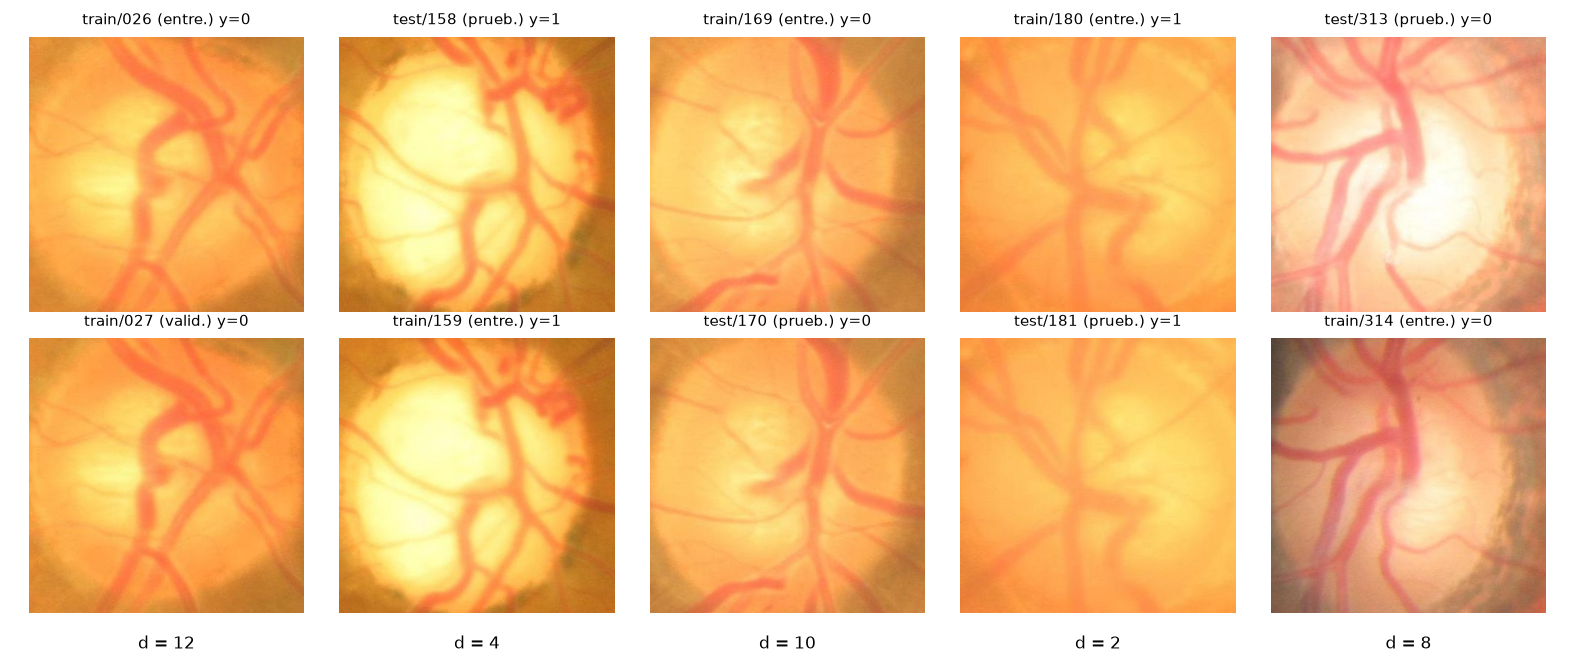
\includegraphics[width=0.85\textwidth]{figuras/pares_mismo_ojo.png}
\caption{Los cinco pares del mismo ojo que cruzan particiones (todas las particiones). Cada columna es un par, con su partición, su etiqueta ($y$) y su distancia pHash ($d$). Los cuatro casos de prueba se excluyen de la evaluación}\label{fig:pares}
\end{figure}

\textbf{Límite declarado.} La guía pide mantener juntos los ojos, las visitas y las repeticiones de una persona. Con esta copia \textbf{no es verificable}: no hay identificador de paciente ni de ojo, y el SERI no respondió la solicitud de la versión oficial. El pHash detecta tomas casi iguales del mismo ojo, pero no los dos ojos de una misma persona, que pueden verse distintos. Por eso no podemos descartar que la prueba contenga el otro ojo de alguien que está en entrenamiento, lo que podría inflar el resultado. Además, todo lo que se aprende de los datos (estandarización, coeficientes, elección de $C$, pesos de la red) se ajusta solo con entrenamiento. La validación se usa para comparar versiones y fijar el umbral, y la prueba se usó una única vez (Sección~\ref{sec:metodo}).

\FloatBarrier
%%==================================================================%%
\section{Método y comparación}\label{sec:metodo}
%%==================================================================%%

\subsection{Flujo y versiones}

La Figura~\ref{fig:flujo} resume el flujo. La línea base es la de la Entrega 2. El \textbf{cambio principal} de las variantes es la representación de la imagen: las 8 medidas hechas a mano se reemplazan por los 512 rasgos que produce una ResNet-18 \cite{he2016resnet} preentrenada en ImageNet \cite{deng2009imagenet}. Esa red se usa como extractor fijo y conserva el mismo clasificador. Así, V1 aísla el efecto de la representación. V2 cambia además la regularización, y V3 deja que la red se adapte a los datos (Tabla~\ref{tab:versiones}).

\begin{figure}[htbp]
\centering
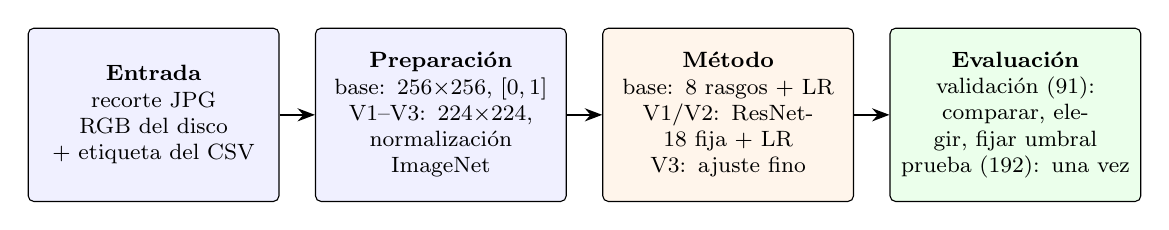
\begin{tikzpicture}[
  caja/.style={draw, rounded corners=2pt, align=center, font=\footnotesize, text width=2.95cm, minimum height=2.2cm, fill=#1},
  caja/.default=white, flecha/.style={-{Stealth[length=2.2mm]}, thick}]
\node[caja=blue!6] (in) {\textbf{Entrada}\\ recorte JPG RGB del disco\\ + etiqueta del CSV};
\node[caja=blue!6, right=0.45cm of in] (pre) {\textbf{Preparación}\\ base: 256$\times$256, $[0,1]$\\ V1--V3: 224$\times$224, normalización ImageNet};
\node[caja=orange!8, right=0.45cm of pre] (met) {\textbf{Método}\\ base: 8 rasgos + LR\\ V1/V2: ResNet-18 fija + LR\\ V3: ajuste fino};
\node[caja=green!8, right=0.45cm of met] (ev) {\textbf{Evaluación}\\ validación (91): comparar, elegir, fijar umbral\\ prueba (192): una vez};
\draw[flecha] (in) -- (pre); \draw[flecha] (pre) -- (met); \draw[flecha] (met) -- (ev);
\end{tikzpicture}
\caption{Flujo de procesamiento: entrada $\rightarrow$ preparación $\rightarrow$ método $\rightarrow$ evaluación. El ajuste usa solo las 363 imágenes de entrenamiento}\label{fig:flujo}
\end{figure}

\begin{table}[htbp]
\small
\caption{Versiones comparadas. Todas se ajustan con las 363 imágenes de entrenamiento y usan la semilla 42}\label{tab:versiones}
\begin{tabularx}{\textwidth}{@{}L{1.1cm}L{4.4cm}YL{3.4cm}@{}}
\toprule
Versión & Representación & Clasificador y parámetros & Cambio frente a la base \\
\midrule
Base & 8 rasgos: media y desviación de R, G y B en el disco (radio 102 px) y palidez centro/anillo en G y R (Entrega 2) & \texttt{StandardScaler} + regresión logística, \texttt{class\_weight="balanced"}, $C=1$ & --- \\
\addlinespace
V1 & 512 rasgos de \textit{avgpool} de ResNet-18 congelada (\texttt{IMAGENET1K\_V1}) & igual que la base ($C=1$) & solo la representación \\
\addlinespace
V2 & igual que V1 & igual, con $C\in\{10^{-6},\dots,1\}$ elegido por CV estratificada de 5 pliegues \textbf{dentro de entrenamiento} (AUC): $C=10^{-4}$ & representación + regularización \\
\addlinespace
V3 & ResNet-18 con \texttt{layer4} y una capa final de 1 salida entrenables & BCE con \texttt{pos\_weight} $=269/94$, AdamW \cite{loshchilov2019adamw} ($\text{lr}=10^{-4}$, \textit{weight decay} $10^{-4}$), lote 16, \textbf{20 épocas fijas} sin \textit{early stopping}; aumento: volteo horizontal, rotación $\pm10^\circ$, brillo y contraste $\pm20\,\%$, recorte de 85--100\,\% & la red se ajusta a los datos \\
\botrule
\end{tabularx}
\end{table}

En V2, la primera grilla de $C$ ($10^{-4}$ a 1) dejó el óptimo de la CV en su extremo inferior. La ampliamos hacia abajo, hasta $10^{-6}$, y el óptimo siguió en $10^{-4}$ (AUC de CV de 0,712). Esa decisión se tomó mirando solo la CV dentro de entrenamiento, pero la declaramos porque ocurrió después de ver la primera ejecución.

\textbf{Protocolo de selección (fijado en \texttt{config.yaml} antes de comparar).}
\begin{enumerate}\raggedright
\item Gana la versión con mayor AUC en las 91 imágenes de validación. Si otra más simple queda a menos de 0,01, gana la más simple. El orden de simplicidad es base $<$ V1 $<$ V2 $<$ V3.
\item El umbral de la elegida es el menor que mantiene en validación una especificidad $\ge 0{,}632$, la de la línea base con umbral 0,5. Así se cumple el criterio secundario anunciado en la Entrega 2: más sensibilidad sin perder especificidad.
\item La versión, el preprocesamiento, el umbral y el SHA-256 de los pesos se guardan en \texttt{version\_elegida.json}.
\item \texttt{11\_evaluacion\_prueba.py} verifica esos hashes, evalúa la prueba y deja un candado (\texttt{prueba\_ejecutada.lock}) que impide repetir la evaluación sin dejar registro.
\end{enumerate}

\textbf{Métricas.} Con glaucoma como positivo: sensibilidad $=$ VP/(VP+FN), especificidad $=$ VN/(VN+FP), F1 de la clase glaucoma y AUC-ROC \cite{fawcett2006roc} sobre la puntuación continua. Para cada métrica damos el intervalo de confianza del 95\,\% por \textit{bootstrap} estratificado por clase (1000 remuestreos, percentiles). La diferencia de AUC frente a la base se estima con un \textit{bootstrap} pareado sobre los mismos casos. Cuando un denominador es cero, la métrica se reporta como no calculable. La exactitud no se usa para decidir, porque el clasificador que siempre responde ``sano'' alcanza 0,747 en validación.

\textbf{Software y equipo.} Python 3.13.2, NumPy 2.5.5, pandas 3.1.1, Pillow 13.0, scikit-learn 1.9.1 \cite{pedregosa2011scikit}, PyTorch 2.15.0 \cite{paszke2019pytorch} y torchvision 0.29.2. Todo corrió en la CPU de un portátil Apple M2 con 8 GB. Extraer los rasgos de las 650 imágenes tarda 14\,s y el ajuste fino de V3, 226\,s. En CPU, con la semilla fija, los resultados se repiten exactamente.

\subsection{Trabajos técnicos de referencia}

\begin{table}[htbp]
\small
\caption{Trabajos técnicos relacionados (actualizada desde la Entrega 2)}\label{tab:estado}
\begin{tabularx}{\textwidth}{@{}L{2.1cm}YYY@{}}
\toprule
Autor y año & Datos y tarea & Método y métrica & Relación con nuestras decisiones \\
\midrule
Cheng et al., 2013 \cite{cheng2013superpixel} & SiMES (650, base de ORIGA) y SCES; segmentación de disco y copa & Superpíxeles con rasgos centro-entorno y CDR. AUC de 0,800 y 0,822 & Motivó la medida de palidez centro/anillo de la base; su ruta necesita contornos que no tenemos \\
\addlinespace
Chen et al., 2015 \cite{chen2015glaucoma} & ORIGA y SCES; glaucoma/sano & CNN de 6 capas entrenada desde cero con aumento de datos. AUC de 0,831 en ORIGA & Con 363 imágenes de entrenamiento descartamos entrenar desde cero y usamos una red preentrenada \\
\addlinespace
Fu et al., 2018 \cite{fu2018denet} & Entrena con ORIGA y prueba en SCES y SINDI & DENet: 4 ramas, entre ellas ResNet-50 sobre la imagen y la región del disco. AUC de 0,918 y 0,817 & Muestra la caída fuera del conjunto de origen; sus ramas necesitan retinografía completa y máscaras \\
\addlinespace
Christopher et al., 2018 \cite{christopher2018transfer} & 14\,822 fotografías del disco de una población diversa; glaucoma/sano & VGG16, Inception-v3 y ResNet-50, con y sin transferencia desde ImageNet. Mejor AUC de 0,91 & La transferencia mejoró todos sus modelos: es la base de nuestro cambio principal (V1--V3) \\
\botrule
\end{tabularx}
\end{table}

Los cuatro trabajos (Tabla~\ref{tab:estado}) sostienen dos decisiones. La primera es concentrarse en la región del disco, que es lo que contienen nuestros recortes. La segunda es usar una red preentrenada en vez de entrenarla desde cero. Christopher et al.\ observaron que la transferencia mejora el desempeño con pocos datos, y Chen et al.\ necesitaron aumento de datos y \textit{dropout} incluso con una red pequeña. Sus cifras son una referencia de lo alcanzable y no una comparación directa, porque usan particiones o versiones de los datos distintas.

\FloatBarrier
%%==================================================================%%
\section{Resultados finales}\label{sec:resultados}
%%==================================================================%%

\subsection{Comparación en validación (91 imágenes: 23 glaucoma, 68 sanas)}

\begin{table}[htbp]
\setlength{\tabcolsep}{3pt}%
\caption{Base y variantes sobre las mismas 91 imágenes de validación, con umbral 0,5. Entre paréntesis, el IC 95\,\%. $\Delta$AUC: diferencia frente a la base (\textit{bootstrap} pareado). AUC ent.: AUC en entrenamiento. Sens.$^{*}$: sensibilidad con el umbral que conserva la especificidad de la base ($\ge 43/68$). Fuente: \texttt{comparacion\_validacion.csv}}\label{tab:comparacion}
\begin{tabular}{@{}lccccccc@{}}
\toprule
Versión & VP/FN/FP/VN & Sens. & Esp. & AUC & $\Delta$AUC & AUC ent. & Sens.$^{*}$ \\
\midrule
Base & 16/7/25/43 & 16/23 = 0,696 & 43/68 = 0,632 & 0,667 (0,54--0,78) & --- & 0,649 & 16/23 \\
V1 & 13/10/11/57 & 13/23 = 0,565 & 57/68 = 0,838 & 0,797 (0,67--0,90) & +0,13 ($-$0,04--0,29) & 1,000 & 21/23 \\
\textbf{V2} & 17/6/16/52 & 17/23 = 0,739 & 52/68 = 0,765 & \textbf{0,831} (0,74--0,91) & +0,16 (0,04--0,31) & 0,810 & 21/23 \\
V3 & 9/14/2/66 & 9/23 = 0,391 & 66/68 = 0,971 & 0,837 (0,73--0,93) & +0,17 (0,01--0,36) & 0,999 & 19/23 \\
\botrule
\end{tabular}
\end{table}

Las tres variantes superan a la base en AUC (Tabla~\ref{tab:comparacion} y Figura~\ref{fig:roccomp}). En V2 y V3, el intervalo de la diferencia queda por encima de cero. V1, con $C=1$, memoriza el entrenamiento (AUC de 1,000 en entrenamiento frente a 0,797 en validación), como anticipamos en la Entrega 2 al pasar de 8 a 512 rasgos. La regularización de V2 elimina ese sobreajuste (0,810 frente a 0,831). V3 también memoriza (0,999) y, con umbral 0,5, apenas detecta 9 de 23 glaucomas: sus puntuaciones no quedan calibradas alrededor de ese valor.

\textbf{Versión elegida: V2.} V3 tiene el AUC más alto (0,837), pero la diferencia con V2 (0,006) es menor que el margen de 0,01. Según la regla, gana la más simple: V2 no necesita entrenar la red, su AUC de entrenamiento no muestra sobreajuste y conserva más sensibilidad con la especificidad de la base (21/23 frente a 19/23). Su umbral congelado es \textbf{0,4834}, que en validación da una sensibilidad de 21/23 y una especificidad de 43/68.

Además, el caso \texttt{train/233}, el falso negativo más marcado de la base ($p=0{,}004$), pasa a $p=0{,}566$ con V2, por encima del umbral. Si se quita \texttt{train/027}, que tiene un gemelo en entrenamiento, los AUC casi no cambian (base 0,665; V2 0,829). La base fallaba más en las tomas claras, con 16 errores de 30 en el tercil más claro. V2 baja a 12 de 30 y V3 a 7 de 30 (Figura~\ref{fig:exposicion}, \texttt{analisis\_comparacion.txt}).

\begin{figure}[htbp]
\centering
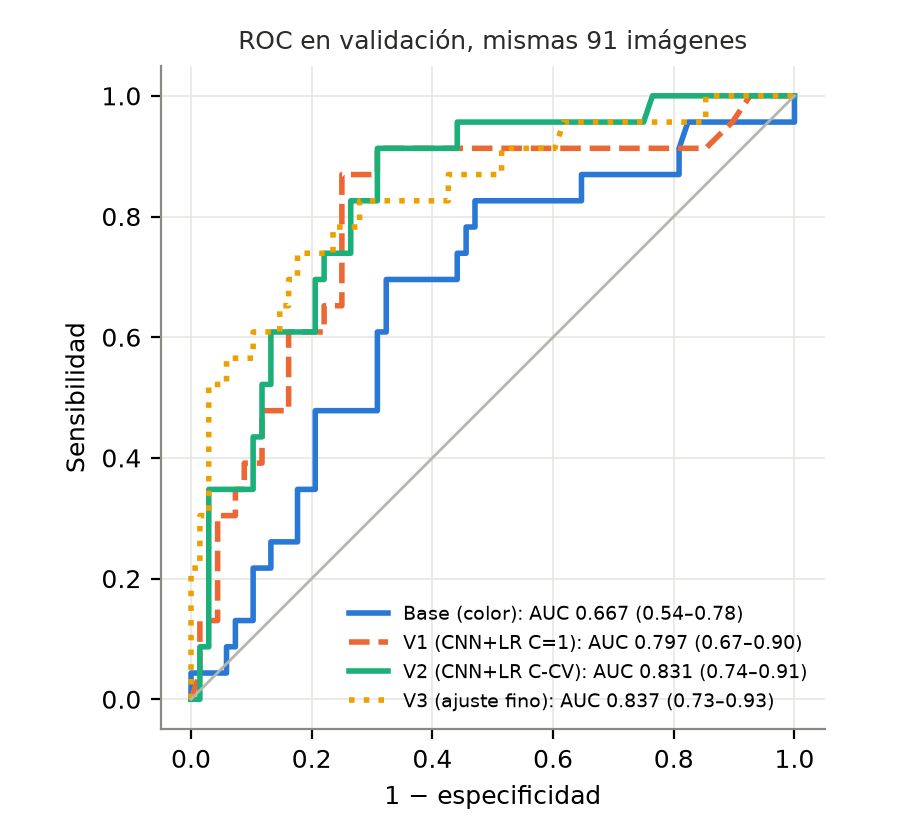
\includegraphics[width=0.47\textwidth]{figuras/roc_comparacion_validacion.png}\hfill
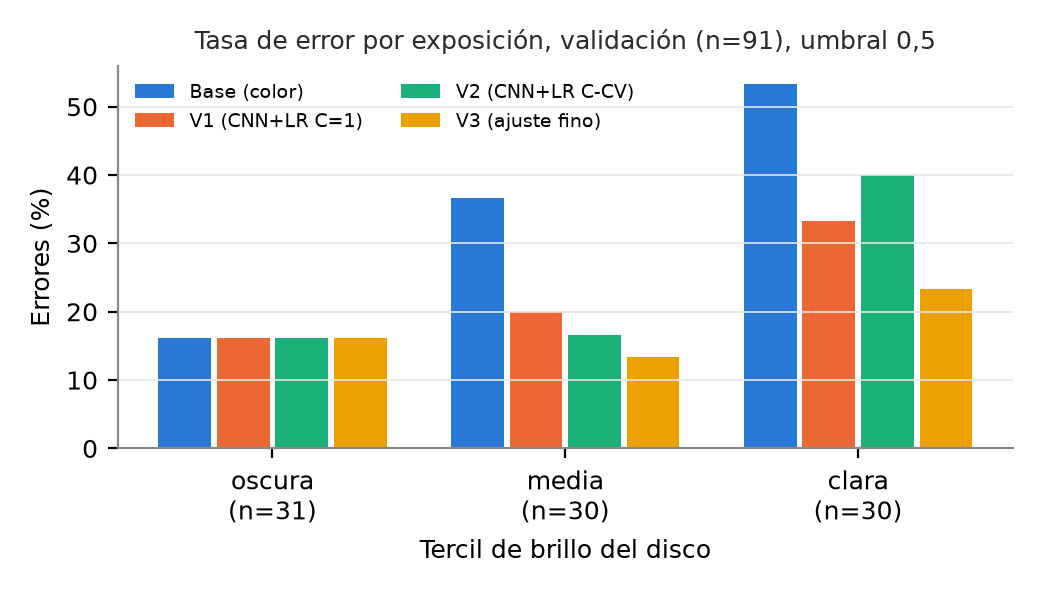
\includegraphics[width=0.51\textwidth]{figuras/errores_exposicion_validacion.png}
\caption{Validación ($n=91$), las cuatro versiones. Izquierda: curvas ROC con AUC e IC 95\,\%. Derecha: tasa de error con umbral 0,5 por tercil de brillo del disco}\label{fig:roccomp}\label{fig:exposicion}
\end{figure}

\subsection{Evaluación en prueba de la versión elegida (V2, umbral 0,4834)}

V2 se aplicó una sola vez, con parámetros, preprocesamiento y umbral congelados, a las 192 imágenes de prueba incluidas (49 con glaucoma y 143 sanas). Las Tablas~\ref{tab:pruebacm} y~\ref{tab:prueba} y la Figura~\ref{fig:prueba} muestran el resultado. Siguiendo la guía, la base no se evaluó en prueba, así que la comparación base/variante se apoya en la validación.

\begin{table}[htbp]
\caption{Matriz de confusión de V2 en prueba ($n=192$), umbral 0,4834. Fuente: \texttt{metricas\_prueba.json}}\label{tab:pruebacm}
\begin{tabular*}{\textwidth}{@{\extracolsep\fill}lcc}
\toprule
 & Predicción: glaucoma & Predicción: sano \\
\midrule
Referencia: glaucoma (49) & VP = 40 & FN = 9 \\
Referencia: sano (143) & FP = 68 & VN = 75 \\
\botrule
\end{tabular*}
\end{table}

\begin{table}[htbp]
\caption{Métricas de V2 en prueba con IC 95\,\% (\textit{bootstrap} estratificado, 1000 remuestreos). Las dos últimas columnas son análisis de sensibilidad del mismo resultado}\label{tab:prueba}
\begin{tabular*}{\textwidth}{@{\extracolsep\fill}lcccc}
\toprule
Métrica & Cálculo & Prueba (192) & Con las 4 excluidas (196) & Sin \texttt{test/175} (191) \\
\midrule
Sensibilidad & 40/49 & 0,816 (0,69--0,92) & 41/51 = 0,804 & 40/49 = 0,816 \\
Especificidad & 75/143 & 0,524 (0,44--0,60) & 77/145 = 0,531 & 75/142 = 0,528 \\
AUC-ROC & puntuación continua & 0,751 (0,66--0,83) & 0,749 & 0,753 \\
F1 (glaucoma) & 80/157 & 0,510 (0,44--0,57) & --- & --- \\
\botrule
\end{tabular*}
\end{table}

\begin{figure}[htbp]
\centering
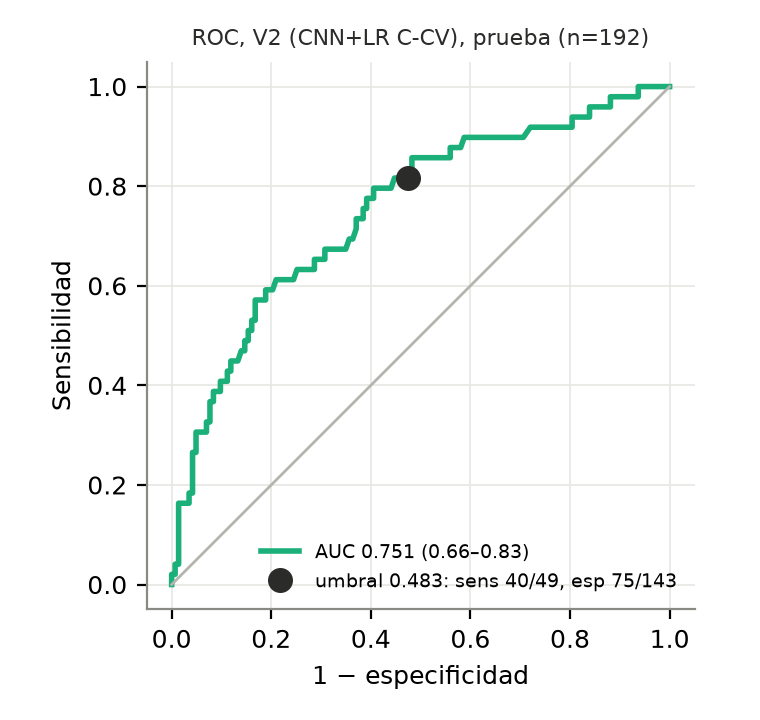
\includegraphics[width=0.42\textwidth]{figuras/roc_prueba.png}\hfill
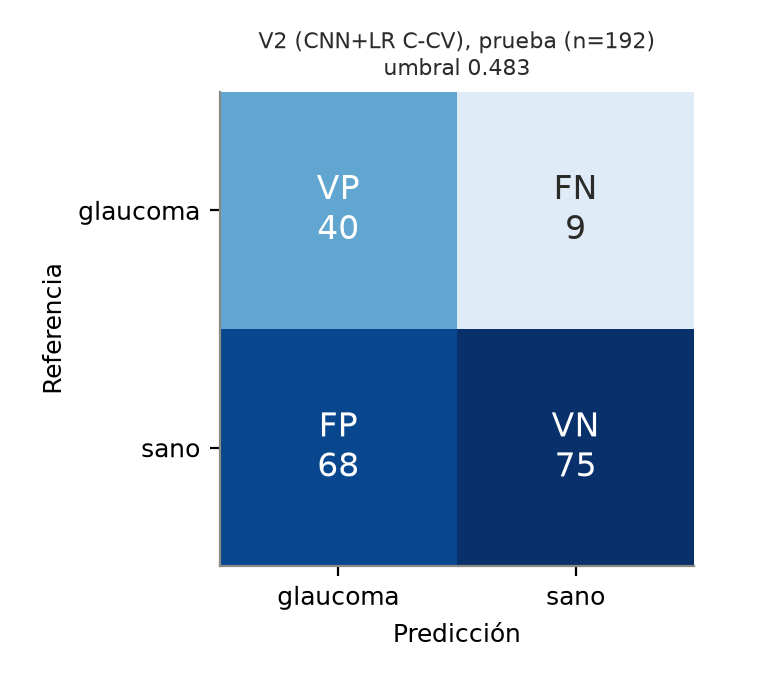
\includegraphics[width=0.42\textwidth]{figuras/matriz_confusion_prueba.png}
\caption{V2 en prueba ($n=192$). Izquierda: curva ROC con el punto de operación congelado. Derecha: matriz de confusión}\label{fig:prueba}
\end{figure}

En prueba, V2 detecta 40 de 49 casos de glaucoma. El precio es alto: 68 de las 143 imágenes sanas se marcan como glaucoma, así que de 108 remisiones, 68 serían falsas alarmas. Frente a la validación, el AUC baja de 0,831 a 0,751 y la especificidad de 43/68 (0,632) a 75/143 (0,524). La sensibilidad baja menos, de 21/23 a 40/49. Los intervalos de validación son anchos, porque solo había 23 positivos, y el AUC de prueba queda apenas dentro del intervalo de validación (0,74--0,91), cerca de su límite inferior. Es decir, la validación sobreestimó el desempeño, algo esperable porque con ella se eligió entre cuatro versiones y se fijó el umbral. Incluir las 4 imágenes excluidas o quitar el par dudoso \texttt{test/175} no cambia el resultado (Tabla~\ref{tab:prueba}).

La Figura~\ref{fig:casos} ilustra cuatro casos de prueba, uno de cada tipo: en cada tipo, el más alejado del umbral. Son solo ejemplos; las métricas se calcularon con las 192 imágenes, cuya tabla por caso está en \texttt{predicciones\_prueba.csv} (Anexo~\ref{secA1}).

\begin{figure}[htbp]
\centering
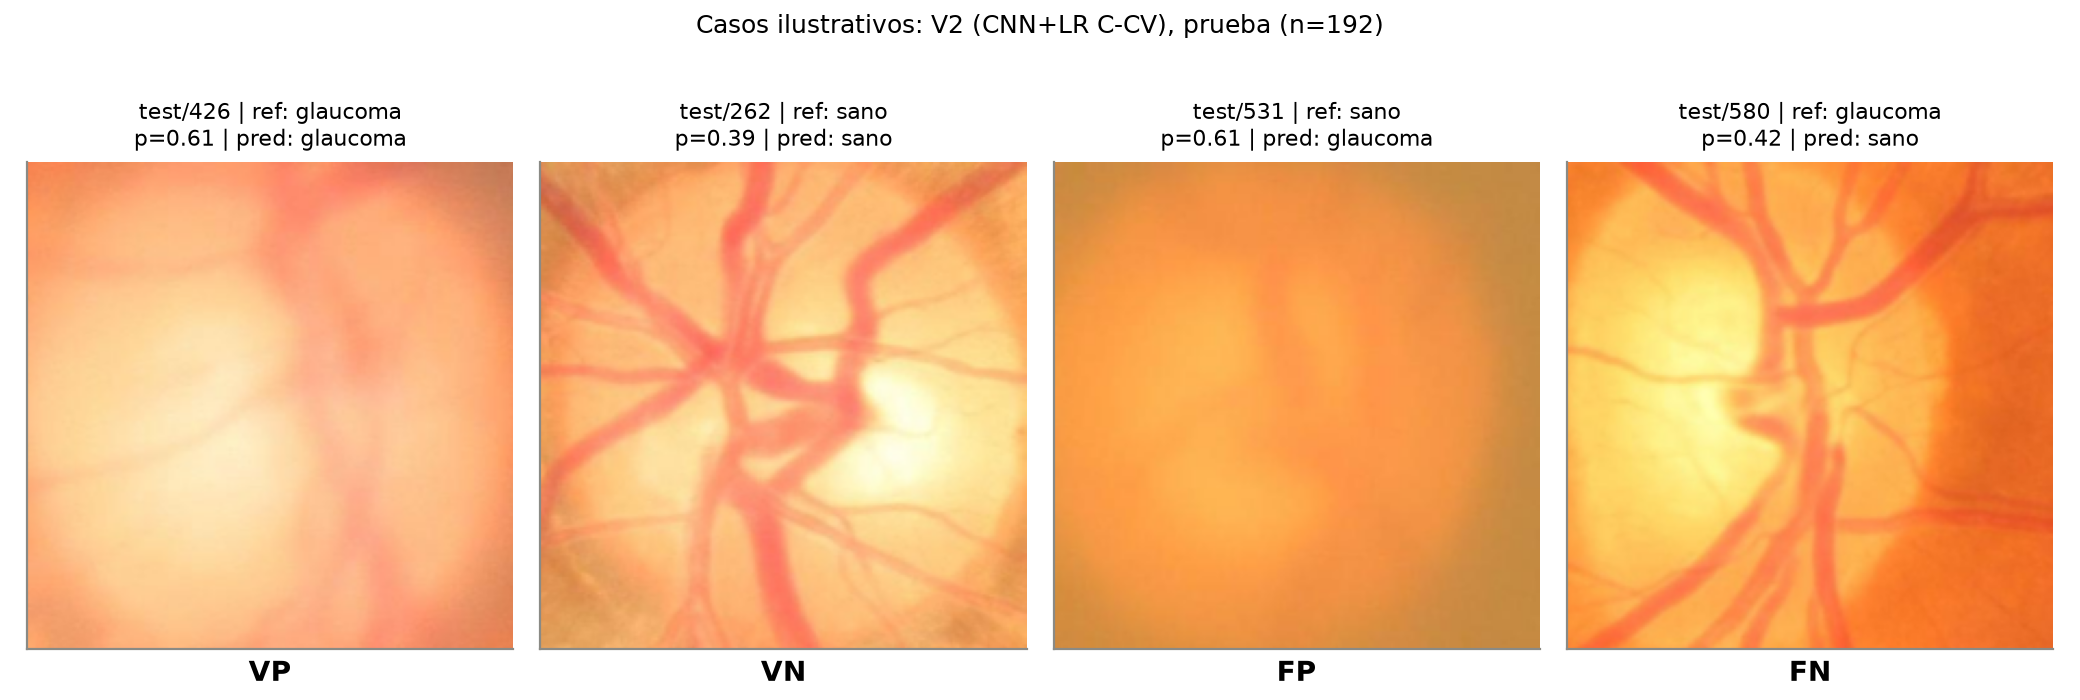
\includegraphics[width=0.9\textwidth]{figuras/casos_prueba.png}
\caption{Casos de prueba ilustrados con V2 (umbral 0,4834; $n=192$): verdadero positivo \texttt{test/426}, verdadero negativo \texttt{test/262}, falso positivo \texttt{test/531} y falso negativo \texttt{test/580}. Sobre cada imagen aparecen el código, la etiqueta de referencia, la puntuación $p$ y la predicción}\label{fig:casos}
\end{figure}

\FloatBarrier
%%==================================================================%%
\section{Errores y limitaciones}\label{sec:errores}
%%==================================================================%%

Analizamos dos casos de la versión final en prueba (Figura~\ref{fig:analizados}): el falso negativo con menor puntuación, porque en tamizaje es el error más costoso, y el caso más cercano al umbral. El mapa Grad-CAM \cite{selvaraju2017gradcam} sobre \texttt{layer4} muestra qué zonas empujan la puntuación hacia glaucoma. Para V2 se calculó derivando la regresión logística a través de la red congelada. Las cifras están en \texttt{analisis\_prueba.txt} y en \texttt{casos\_analizados\_prueba.csv}.

\begin{figure}[htbp]
\centering
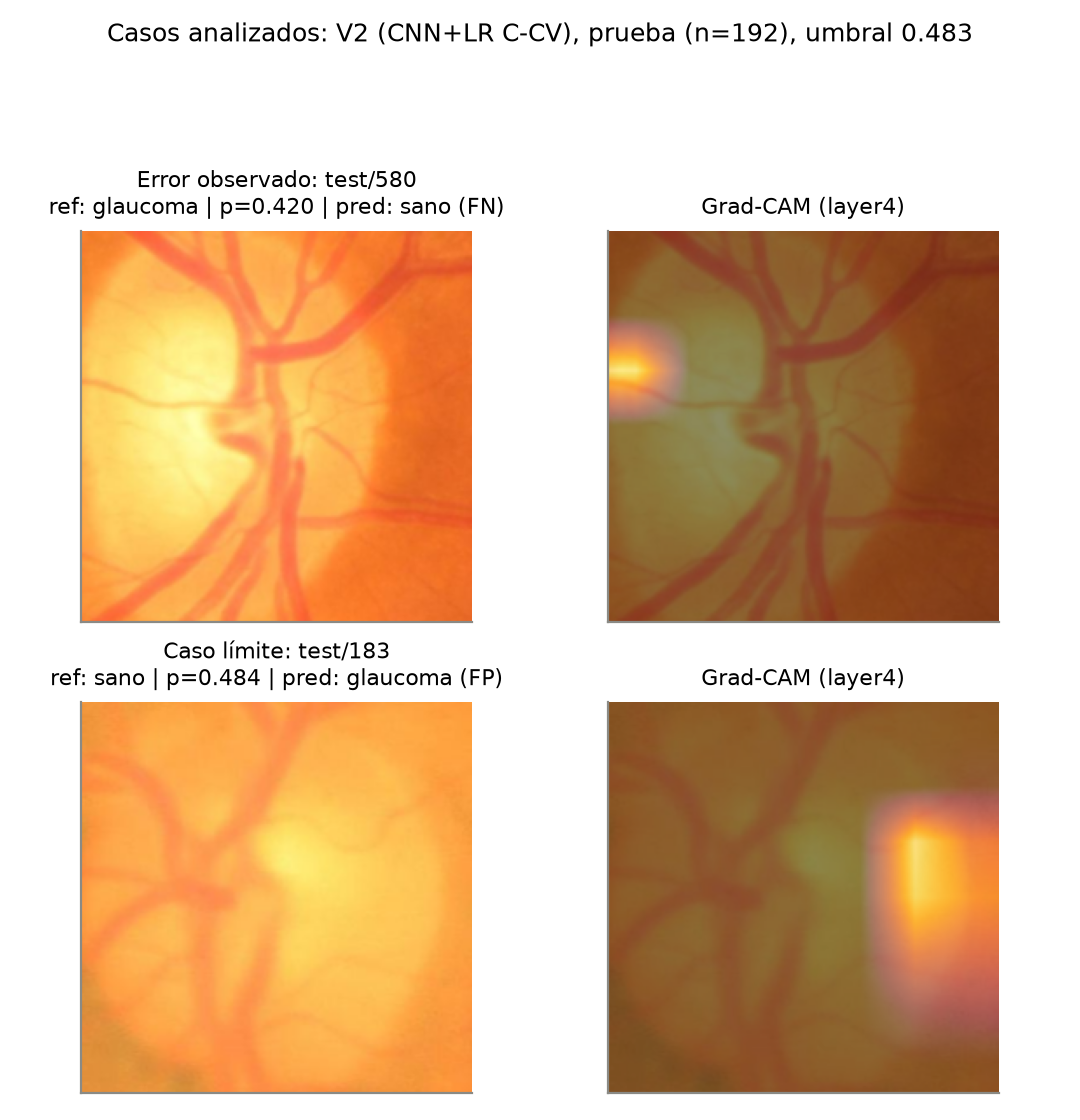
\includegraphics[width=0.72\textwidth]{figuras/casos_analizados_prueba.png}
\caption{Casos analizados de V2 en prueba (umbral 0,4834; $n=192$). Arriba: error observado, \texttt{test/580}, un falso negativo. Abajo: caso límite, \texttt{test/183}, un falso positivo a 0,0001 del umbral. A la derecha, el mapa Grad-CAM superpuesto}\label{fig:analizados}
\end{figure}

\needspace{6\baselineskip}
\textbf{Caso 1: error observado (\texttt{test/580}).}
\begin{itemize}
\item \textbf{Referencia y salida:} glaucoma; $p=0{,}420$, predicción sano (FN), a 0,064 por debajo del umbral. Es el FN más alejado del umbral. Los otros 8 FN están entre 0,437 y 0,482.
\item \textbf{Qué se observa:} el disco no está centrado en el recorte. Ocupa la mitad izquierda, con una zona central amplia y pálida y vasos que la cruzan, mientras que la mitad derecha es retina naranja oscura. El brillo del disco es típico (percentil 44 de la prueba), así que la exposición no explica este error, a diferencia de \texttt{train/233} en la base. El Grad-CAM se concentra en el borde izquierdo y no en la zona pálida central.
\item \textbf{Hipótesis (no demostrada):} los rasgos de ImageNet, promediados sobre toda la imagen, mezclan el disco con la retina de alrededor. Cuando el disco está descentrado, la mitad de los rasgos describe retina sin información sobre la copa, y la puntuación se acerca a la de un ojo sano.
\item \textbf{Cómo comprobarla:} recentrar el recorte en el disco (por ejemplo, en el máximo de brillo suavizado), volver a puntuar sin reentrenar y ver si este caso y los demás FN suben. También se puede repetir el Grad-CAM sobre los 9 FN para ver si la atención cae fuera del disco.
\end{itemize}

\needspace{6\baselineskip}
\textbf{Caso 2: caso límite (\texttt{test/183}).}
\begin{itemize}
\item \textbf{Referencia y salida:} sano; $p=0{,}4836$, predicción glaucoma (FP). Queda a 0,0001 del umbral, de modo que cualquier variación mínima cambiaría la clase.
\item \textbf{Qué se observa:} la toma está desenfocada y los vasos y el borde del disco se ven difusos. El centro es claro y amarillento. El Grad-CAM marca la retina del borde derecho.
\item \textbf{Hipótesis:} sin bordes nítidos, los rasgos pierden la información de forma, y la puntuación cae en la zona de máxima mezcla de las dos clases.
\item \textbf{Lectura general:} este caso refleja el problema que explica la caída de especificidad. Con $C=10^{-4}$, las puntuaciones de V2 quedan comprimidas entre 0,39 y 0,61, y la mediana de las sanas en prueba es 0,48, prácticamente igual al umbral. De los 68 FP, 45 tienen $p<0{,}52$.
\item \textbf{Análisis exploratorio, sin usarlo para decidir:} con umbral 0,5 la prueba habría dado una sensibilidad de 33/49 y una especificidad de 95/143. El punto de operación es muy sensible a un desplazamiento pequeño del umbral, y fijarlo con solo 91 imágenes lo vuelve frágil.
\end{itemize}

\needspace{6\baselineskip}
\textbf{Límites del estudio.}
\begin{enumerate}
\item \textbf{Independencia:} sin identificador de paciente no se puede garantizar que una misma persona no esté en dos particiones (Sección~\ref{sec:particion}).
\item \textbf{Un solo origen:} todas las imágenes provienen del estudio SiMES, con población malaya, la misma cámara y criterios homogéneos. Fu et al.\ muestran que el desempeño baja al cambiar de población \cite{fu2018denet}.
\item \textbf{Etiquetas:} un par del mismo ojo tiene etiquetas opuestas, y la etiqueta clínica integra información (presión, campo visual) que la foto no contiene.
\item \textbf{Tamaño:} con 23 positivos en validación y 49 en prueba, los intervalos son anchos (AUC de prueba entre 0,66 y 0,83). Por eso no distinguimos entre V2 y V3.
\item \textbf{Datos de entrada:} recortes JPG ya comprimidos y sin máscaras; no pudimos evaluar la ruta basada en la relación copa/disco.
\item \textbf{Interpretación:} el Grad-CAM de los casos analizados no muestra que el modelo use la copa óptica, así que no podemos afirmar que reconozca el signo clínico.
\end{enumerate}

\FloatBarrier
%%==================================================================%%
\section{Conclusiones y aportes}\label{sec:conclusiones}
%%==================================================================%%

\textbf{Respuesta a la pregunta.} Con esta copia de ORIGA-light, sí es posible identificar glaucoma \emph{por encima del azar}. La versión final obtuvo en prueba, sobre 192 imágenes nunca usadas para ajustar, un AUC de 0,751 (IC 95\,\%: 0,66--0,83) y detectó 40 de 49 casos. No es posible hacerlo con la especificidad que exigiría un tamizaje: solo 75 de 143 imágenes sanas se clasificaron como sanas.

\textbf{Qué mejoró.} En las mismas 91 imágenes de validación, cambiar las medidas de color por rasgos de ResNet-18 subió el AUC de 0,667 a 0,831 (+0,16; IC 0,04--0,31). También corrigió el falso negativo extremo de la base (\texttt{train/233}) y redujo su dependencia de la exposición. Regularizar fue necesario: sin regularización (V1), el modelo memorizó el entrenamiento.

\textbf{Qué no mejoró.} El ajuste fino (V3) no superó a V2 por un margen relevante y memorizó el entrenamiento. En prueba, la especificidad cayó por debajo de la que buscábamos (0,524 frente a 0,632), porque las puntuaciones de V2 están muy concentradas alrededor del umbral.

\needspace{6\baselineskip}
\textbf{Qué no puede concluirse.}
\begin{itemize}
\item La utilidad clínica.
\item El desempeño en otras poblaciones o cámaras.
\item Que el modelo use la copa óptica.
\item Que V2 sea mejor que V3, porque sus intervalos se solapan.
\item La ventaja de V2 sobre la base \emph{en prueba}, porque la base no se evaluó allí.
\end{itemize}

\textbf{Limitación prioritaria para trabajo futuro.} Obtener la versión oficial con identificador de paciente y ojo, para repetir la partición agrupando por persona y validar en un conjunto externo (por ejemplo, REFUGE). Con más datos de validación también se podría fijar un umbral menos frágil.

\begin{table}[htbp]
\small
\caption{Aportes verificables de cada integrante en la entrega final}\label{tab:roles}
\begin{tabularx}{\textwidth}{@{}L{2.7cm}YY@{}}
\toprule
Integrante & Tarea & Evidencia (ZIP) \\
\midrule
Giuseppe Kanyike Buwule & Actualizó la sección de datos y partición, la tabla de trabajos relacionados y comprobó que los conteos del informe coinciden con los archivos & Tablas~\ref{tab:datos}, \ref{tab:particion} y~\ref{tab:estado}; \texttt{particion\_final.csv}, \texttt{metricas\_prueba.json} \\
Daniel Duque & Analizó los errores de la versión final (casos \texttt{test/580} y \texttt{test/183}, exposición) y redactó la discusión y las conclusiones & Secciones~\ref{sec:errores} y~\ref{sec:conclusiones}; \texttt{analisis\_prueba.txt}, \texttt{casos\_analizados\_prueba.csv} \\
Juan David Daza & Implementó y ejecutó las variantes, la comparación, la evaluación única en prueba y la inferencia; armó el informe y el ZIP & \texttt{07}--\texttt{13\_*.py}, \texttt{modelos.py}, \texttt{predecir.py}, \texttt{version\_elegida.json}, \texttt{prueba\_ejecutada.lock} \\
\botrule
\end{tabularx}
\end{table}

\FloatBarrier
\backmatter

\bmhead{Uso de herramientas}

Usamos Claude (Anthropic) \cite{anthropic2026claude} mediante Claude Code para programar los scripts y redactar borradores de este informe. Verificamos su salida así:
\begin{itemize}
\item ejecutamos todo el código;
\item comprobamos que la línea base de la Entrega 2 se reproduce de forma idéntica;
\item cotejamos cada cifra del texto con los JSON, CSV y TXT de \texttt{resultados/};
\item revisamos a ojo cada figura.
\end{itemize}
El documento sigue la plantilla \LaTeX\ de Springer Nature \cite{springer2024latex}.

\bibliography{referencias}

\clearpage
\begin{appendices}

\section{Resultados por caso en prueba}\label{secA1}

La tabla completa por caso de prueba está en \texttt{predicciones\_prueba.csv}. Tiene una fila por cada una de las 196 imágenes, con su código, partición, versión, etiqueta, puntuación, umbral, predicción, tipo e inclusión en la evaluación. La Tabla~\ref{tab:errores} lista los 77 errores de las 192 imágenes evaluadas; los 115 aciertos son 40 VP y 75 VN. Las tablas equivalentes de validación para las cuatro versiones están en \texttt{predicciones\_validacion\_todas.csv}.

\begin{table}[htbp]
\small
\caption{Errores de V2 en prueba ($n=192$, umbral 0,4834): número de imagen (\texttt{test/}) y, entre paréntesis, la puntuación, de menor a mayor}\label{tab:errores}
\begin{tabularx}{\textwidth}{@{}L{2.2cm}Y@{}}
\toprule
Tipo & Casos \\
\midrule
FN (9): glaucoma predicho como sano & 580 (0,420), 317 (0,437), 229 (0,446), 116 (0,450), 246 (0,460), 601 (0,473), 480 (0,475), 289 (0,481), 514 (0,482) \\
\midrule
FP (68): sano predicho como glaucoma & 183 (0,484), 254 (0,484), 179 (0,484), 423 (0,485), 384 (0,485), 504 (0,487), 332 (0,487), 434 (0,488), 347 (0,488), 091 (0,488), 401 (0,489), 577 (0,491), 123 (0,492), 257 (0,493), 268 (0,493), 251 (0,495), 173 (0,498), 581 (0,499), 501 (0,499), 358 (0,500), 418 (0,501), 343 (0,501), 054 (0,501), 299 (0,502), 040 (0,502), 566 (0,503), 152 (0,503), 430 (0,506), 095 (0,506), 098 (0,507), 178 (0,507), 393 (0,507), 315 (0,507), 583 (0,508), 002 (0,509), 162 (0,509), 428 (0,510), 522 (0,511), 236 (0,511), 292 (0,512), 124 (0,513), 309 (0,514), 568 (0,515), 406 (0,515), 239 (0,519), 175 (0,522), 449 (0,523), 620 (0,526), 034 (0,527), 367 (0,528), 258 (0,528), 561 (0,528), 344 (0,531), 205 (0,533), 540 (0,533), 215 (0,534), 574 (0,536), 629 (0,541), 265 (0,545), 492 (0,547), 197 (0,549), 438 (0,555), 276 (0,573), 355 (0,576), 610 (0,576), 232 (0,577), 594 (0,606), 531 (0,609) \\
\botrule
\end{tabularx}
\end{table}

\FloatBarrier
\section{Contenido del ZIP de evidencias y cómo ejecutarlo}\label{secA2}

El archivo \texttt{EF\_Proyecto\_B\_Equipo02\_2026-30\_Evidencias.zip} contiene:

{\raggedright
\begin{itemize}\raggedright
\item \texttt{README.md}: software y versiones, instalación, estructura, ruta de datos, semilla, secuencia exacta de ejecución y salidas esperadas.
\item \texttt{codigo/}: \texttt{config.yaml} (parámetros de la base y las variantes, regla de selección y revisión visual), \texttt{requirements.txt}, \texttt{comun.py}, \texttt{modelos.py}, los scripts \texttt{01}--\texttt{13} y \texttt{predecir.py}.
\item \texttt{codigo/modelos/}: pesos entrenados (\texttt{modelo\_base.joblib}, \texttt{modelo\_v1.joblib}, \texttt{modelo\_v2.joblib}, \texttt{modelo\_v3.pt}). Los pesos de ImageNet de ResNet-18 se descargan del enlace oficial de torchvision.
\item \texttt{codigo/resultados/}: inventario y partición (\texttt{inventario.csv}, \texttt{particion\_final.csv}, \texttt{verificacion\_particion.txt}, \texttt{revision\_pares.csv}, \texttt{prueba\_excluidos.csv}); validación (\texttt{comparacion\_validacion.csv}, \texttt{predicciones\_validacion\_todas.csv}, \texttt{metricas\_validacion*.json}, \texttt{version\_elegida.json}); prueba (\texttt{predicciones\_prueba.csv}, \texttt{metricas\_prueba.json}, \texttt{prueba\_ejecutada.lock}); análisis (\texttt{analisis\_comparacion.txt}, \texttt{analisis\_prueba.txt}).
\item \texttt{codigo/figuras/}: todas las figuras de este informe y las de la Entrega 2.
\item \texttt{Presentacion.pdf}: diapositivas de la sustentación.
\end{itemize}
}

El conjunto de datos no se incluye: se descarga de Kaggle y se ubica según \texttt{config.yaml}. El entrenamiento (\texttt{07}--\texttt{09}, unos 4 minutos en CPU) está separado de la evaluación y la inferencia (\texttt{10}--\texttt{13} y \texttt{predecir.py}), que usan los pesos incluidos. Ejemplo de inferencia: \texttt{python predecir.py ../archive/ORIGA/test/580.jpg}.

\end{appendices}

\end{document}
